% !TEX root = ../rawlik-phd-thesis.tex
\chapter{Axion analysis}
\label{ch:axion-analysis}

Now that the foundation of the analysis has been introduced, we describe how it was applied to look for oscillations in the neutron EDM data taken at the PSI in the years 2015--17.

First we considered the scalar coupling, acting like an oscillating nEDM signal. We analysed directly the time series of $R$, measured with every cycle of the experiment. This allowed us to consider frequencies up to inverse \SI{300}{\second}, but, on the other hand, required a careful consideration of the effect that on oscillating nEDM would would have on the $R$ time series. Not having found a signal, we could interpret this analysis as the first laboratory limits on the axion coupling to gluons.

The work described in this chapter was a joint effort with Nicholas Ayres, who analysed the data of the Grenoble-based nEDM measurement~\cite{AyresThesis} in search for the scalar coupling. Rather than the raw $R$ time series, he considered the one of the nEDM estimates as obtained on a run basis. The two analyses were complimentary, each covering a different range of oscillation frequencies.

Then we discuss a different coupling, a vector one, acting like on oscillating magnetic field. No significant discovery could be claimed here, which led to exclusions for the axion-nucleon coupling.

Finally, we considered a particular frequency of \num{23.934}~hours, the sidereal frequency.
\marginpar{The sidereal frequency is the one of the Earth spinning in the celestial coordinates.}
Oscillations of that periodicity can be interpreted a hint of a \emph{cosmic spin anisotropy field}~\cite{Altarev2009}.



\section{How a signal would look like}
We start by considering, how an oscillating electric dipole moment would have come up in the $R$ time series, as measured by the PSI experiment.

The main purpose of the experiment was to measure the static neutron electric dipole moment. This would appear as a shift in $R$ dependent on direction of the electric field relative to the magnetic one. In a zero electric field there would be no shift, while the parallel and anti-parallel configurations of the magnetic and electric fields would shift $R$ in opposite directions. Due to the data blinding
% \footnote{In order to reduce bias the data were modified upon being taken in a way, that a secret nEDM was injected into them. This additional offset is only revealed as the very last step, once the measurement and analysis have been completed. The data were still blinded at the time of writing.}
we expect a pronounce shift corresponding to an nEDM of \SI{e-25}{\elementarycharge\centi\meter}.

Should the neutron electric dipole moment oscillate, $R$ would oscillate as well, even if the electric field is kept constant. A reversal of the electric field polarity would reverse the phase of the oscillations. At zero electric field no oscillations would be visible. In the PSI experiment the field was automatically changed according to the looped pattern: 48 cycles in one polarity, 8 cycles without the field, 48 cycles in the other, 8 without the field. In Fig.\,\ref{fig:axions_data_taking_one_run} we depict an $R$ time series with the combined effect of a large nEDM oscillation and the blinding offset.

\begin{figure}
  \centering
  \subfloat[An oscillating neutron electric dipole moment signal in the nEDM @ PSI apparatus. The colours indicate different electric field states: parallel to the magnetic field, antiparallel to it and zero]
  {\label{fig:axions_data_taking_one_run}
  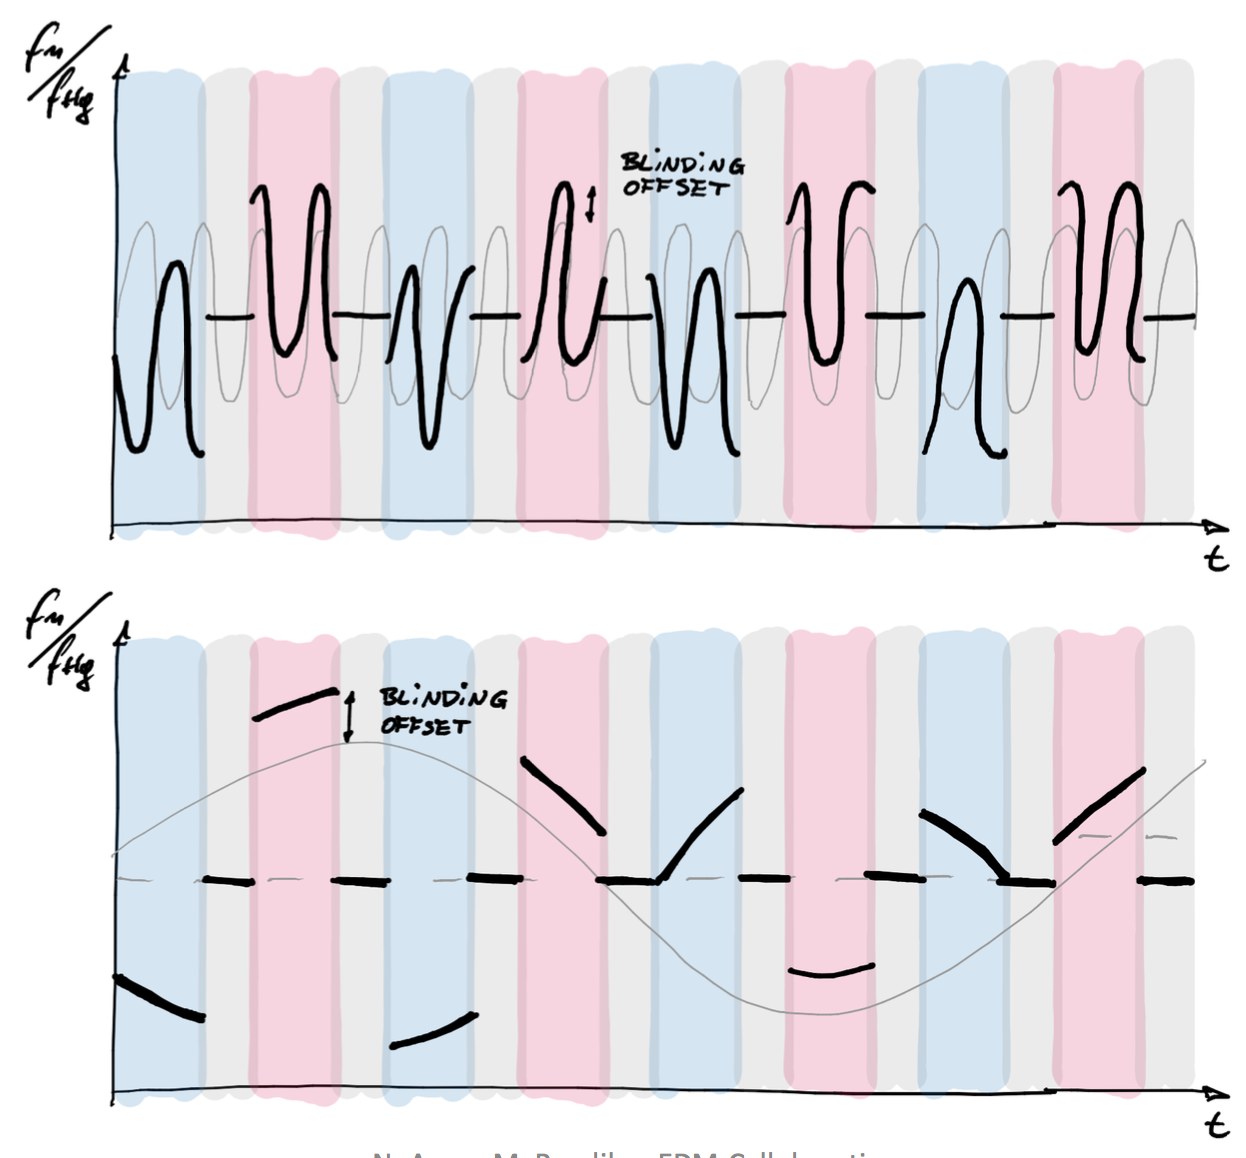
\includegraphics[width=.34\linewidth]{gfx/axions/cycle-level_blinding_offset.png}}
  \quad
  \subfloat[An oscillating neutron electric dipole moment signal in the nEDM @ PSI apparatus across many runs. The colours indicate different electric field states: parallel to the magnetic field, antiparallel to it and zero. Different runs have different magnetic field gradients, which causes each run to have a different shift in $R = f_n / f_{Hg}$.]
  {\label{fig:axions_data_taking_runs}
  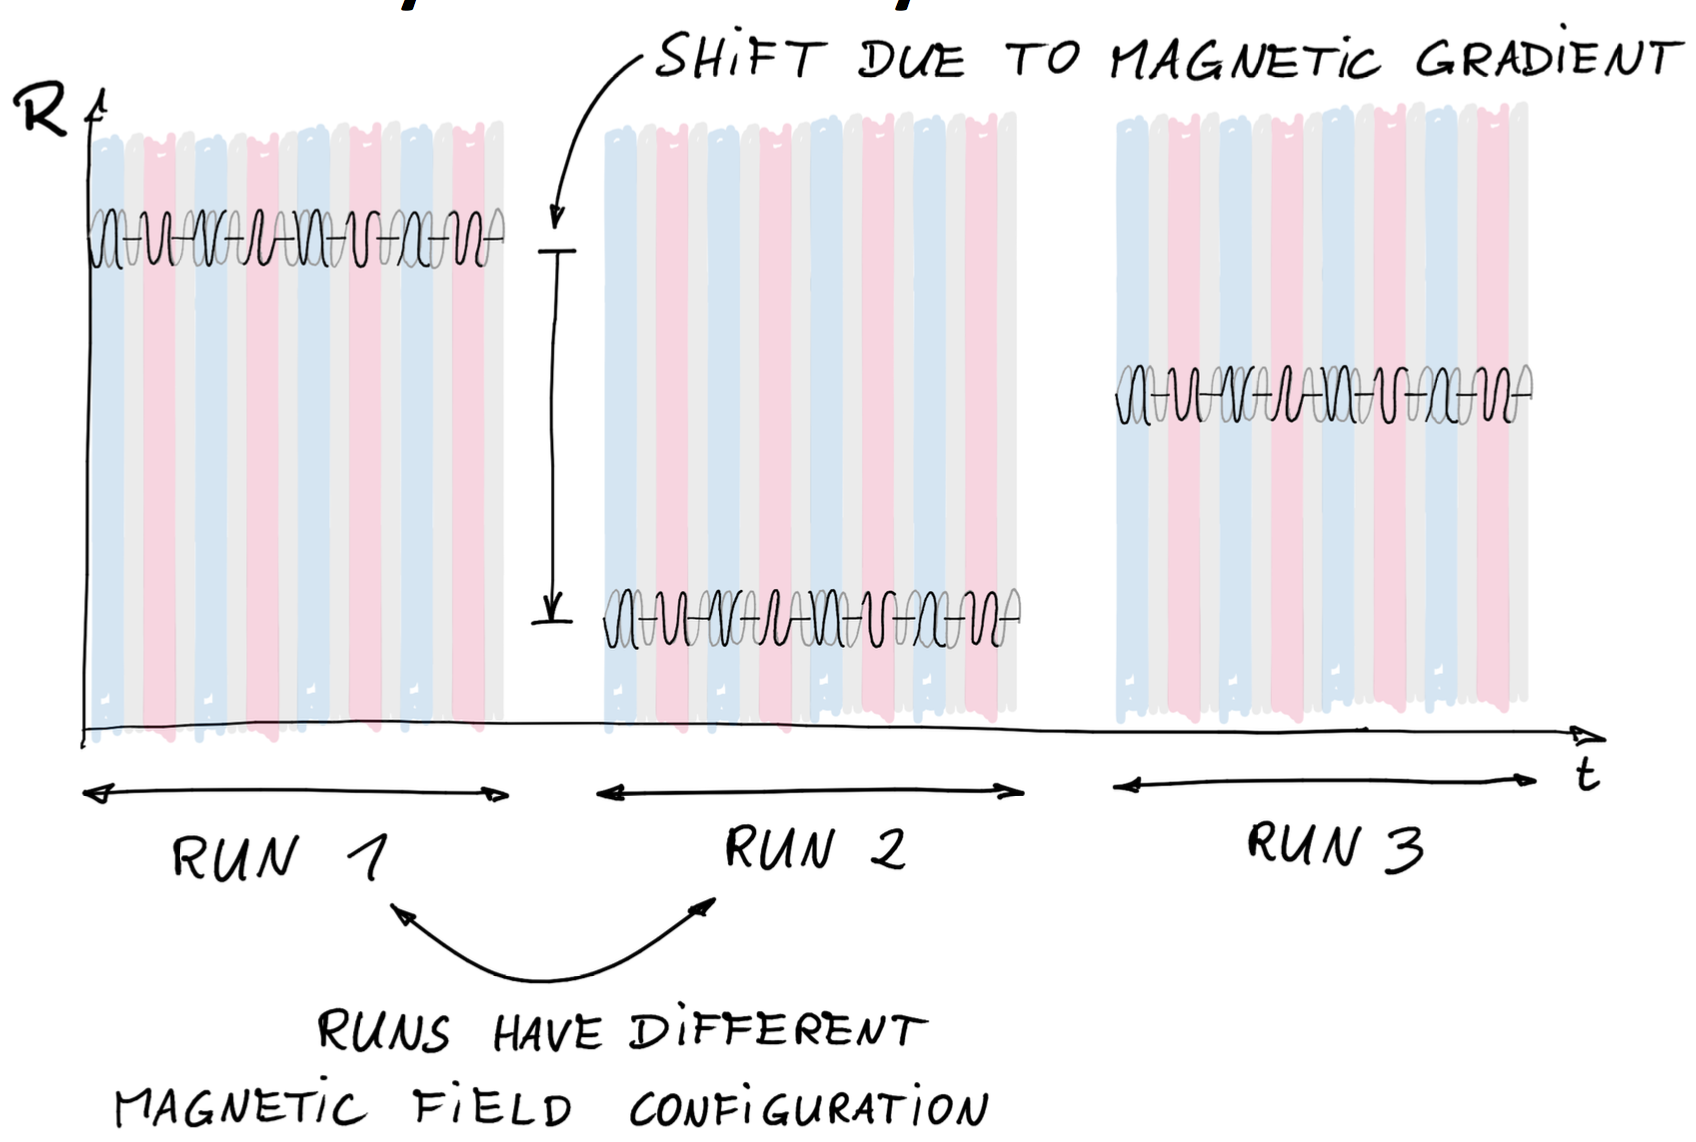
\includegraphics[width=.56\linewidth]{gfx/axions/cycle-level_gradient_jump.png}}
  \caption{The data taking scheme in the nEDM experiment at PSI.}
\end{figure}

Of course, the least-squares spectral analysis could not be applied directly to the complicated $R$ time series. Note, that the time series is still a part of a harmonic oscillation, when only one electric field polarity is considered. Or, to be exact, one relative configuration of the electric and magnetic fields. In the analysis the $R$ time series was split according to this condition into three: one without the electric field (not sensitive to an oscillation of nEDM), one with the electric and magnetic fields parallel and one with anti-parallel. The last having the hypothetical oscillation in the opposite phase then the parallel one. We will refer to the three data sets as $E=0$, $E \uparrow \uparrow B$ and $E \uparrow \downarrow B$, respectively. Each of those was treated separately.

% \begin{figure}[bth]
%   %FIXME directly copied from Elise's presentation on the 2015 PSI collaboration meeting
%   \myfloatalign
%   \subfloat
%   [Another time series of $R$ in the nEDM experiment. The colours depict electric field states, black being no electric field. A drift is clearly visible.]
%   {\label{fig:axions_gradient_drift_not_corrected}
%   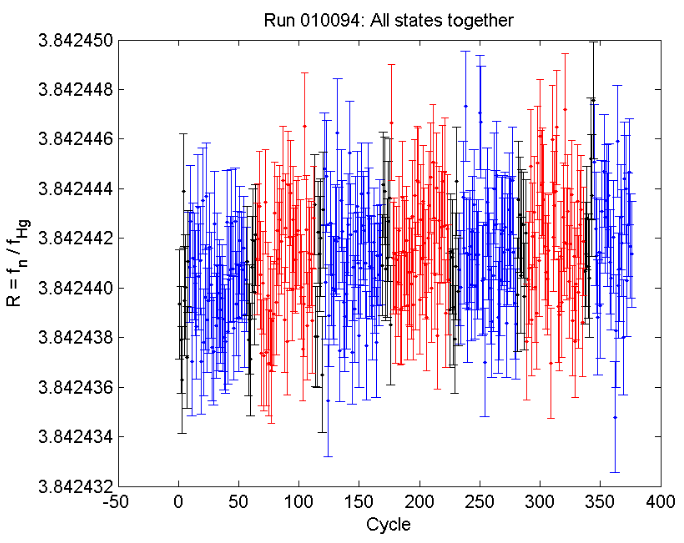
\includegraphics[width=.45\linewidth]{gfx/axions/gradient_drift_elise}}
%   \quad
%   \subfloat
%   [The data as on Fig.\,\ref{fig:axions_gradient_drift_not_corrected} corrected for gradient fluctuations.]
%   {\label{fig:axions_gradient_drift_corrected}
%   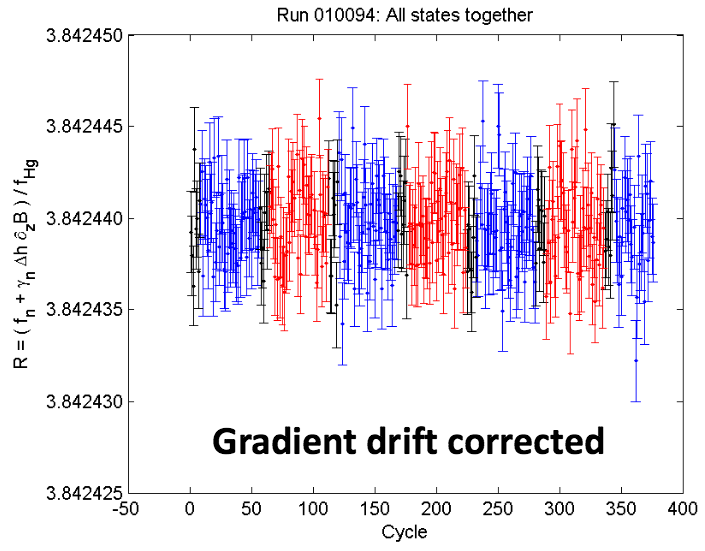
\includegraphics[width=.45\linewidth]{gfx/axions/gradient_drift_elise_corrected}}
%   \caption{Correcting the $R$ time series for fluctuations of the vertical magnetic field gradient.}
%   \label{fig:axions_gradient_drift_correction}
% \end{figure}

There are other effects in the $R$ time series. A part of the measurement procedure was to deliberately work in a magnetic field gradient, as discussed in Sec.\,\ref{sec:measurement_procedure}. The vertical magnetic field gradient changed substantially between sequences. Thereby $R$ was affected by a big value, changing the DC level of the oscillating nEDM signal, as illustrated in Fig.\,\ref{fig:axions_data_taking_runs}.

The problem of inter-sequence jumps was solved by allowing the DC offset in the LSSA fit to be different in each sequence:
\begin{equation}
  \label{eq:axions_LSSA}
  A\sin(2 \pi f t) + B\cos(2 \pi f t) + \sum_i C_i\,\Pi_i(t) \ ,
\end{equation}
where $C_i$ is the free offset in the $i$th sequence and $\Pi_i(t)$ is a gate function equal to one in the $i$th sequence and zero elsewhere. In this way the model explicitly assumed coherence of the oscillation across sequences. However, the downside was a reduced sensitivity to oscillations slower than a sequence (2--3 days), as they could be absorbed into the different free offsets. This, together with the split into three series, reduced the problem to one described in the previous chapter.

% It may be tempting to think about demodulating the $R$ time-series into what would be expected to be an oscillation. This would require subtracting the DC offset for each electric field configuration, in each run separately, then flipping the signal around the DC level for one configuration. \mnote{The offsets are measured with Cs, mention that.} The disadvantage is that uncertainty in such a demodulation would become a systematic effect and would need to be tightly controlled.

% , as clearly visible in Fig.\,\ref{fig:axions_gradient_drift_correction}.
% The nEDM team spares no effort to measure the gradient. Nevertheless, the achieved precision (\SI[per-mode=symbol]{\approx 1}{\pico\tesla\per\centi\meter}) is only comparable to the one of $f_n$ (in the order of \SI{1}{\pico\tesla}). The exact way how the gradient should determined is highly non--trivial and there is ongoing research in this respect. \mnote{Mention here the exact way the gradient drift correction is done. And cite Elise's thesis.} Actually, even the height difference between the neutrons and $^{199}$Hg centres of mass (a few millimeters) is still discussed. \mnote{Know how exactly was $\Delta h$ determined in the end. Also, mention the definition of a sequence here (as in the paper).}
% \cite{Afach2014magmoment}

% Assuming a constant gradient during a \emph{run} one can determine it much more precise. This assumption, however, is known not to be exactly true.

% One should note, that any, including an oscillating one, nEDM effect affects only the position of the neutrons' resonance. The shape of the resonance curve is unaffected. Therefore, the method to extract neutron Larmor frequency $f_n$, and thereby $R$, for each \emph{cycle} is valid also in case of an oscillating nEDM.



\section{Systematic Effects}
In the analysis the compatibility of the periodogram of the $R$ time series with the one of pure noise, the null hypothesis, was tested. Variations in $R$, harmonic in particular, but not only, would have resulted in an additional power in the periodogram and could, therefore, be considered a systematic effect.

Most prominently, $R$ followed the changes in the vertical gradient of the magnetic field. Because of the centre of height difference between the neutron and mercury atom ensembles they saw, on average, a different field in a presence of the vertical gradient.  Luckily, it could be corrected for with the use of the cesium magnetometers. On a cycle basis, a second-order parametrisation of the field was fitted to their readouts, giving an estimate of the gradient~\cite{Afach2014magmoment,WurstenThesis}. Due to unknown random offsets in the magnetometers' readings the correction was only relative---correcting for the variations of the gradient. In between runs the caesium magnetometers were calibrated, which altered the offsets. For this reason the correction could not extend across a run boundary. 
% , which changed in between runs which changing after this correction could only be relative in a run.
% \marginpar{STILL CHANGE RUN TO SEQUENCE!!!}

There could have been, potentially, other effects causing the time series of $R$ not to be fully random. An important decision had to be taken on how to treat those. Two possibilities were considered.

A detail study of time-dependent systematic effect could be performed.
Here any excess in power, in any dataset ($E \uparrow \uparrow B$, $E \uparrow \downarrow B$ and $E=0$) would be treated as a signature of some kind of a signal. All effects that could potentially result in that would have to be identified before the analysis was performed and corrected for. This would have required a long and careful systematic study. Moreover, the full-fledged systematic studies for the constant nEDM analysis of the PSI data were still ongoing at the time. This approach was considered to be, albeit careful, not necessary for this analysis.

% \paragraph{Determine delicate frequencies and cut them out.}
% The experiment run 
% Looking at periodograms of raw data one sees that there are several typical frequencies where peaks appear. Typically at inverse specific time constants at which the experiment operates: cycle separation, day, week, , HV-reversal, B0-reversal. We may decide that all systematic effects are constrained to these frequencies and do not perform the analysis there at all.

% \paragraph{Assume there are no systematic effects.}
Instead, an easier approach was taken. An axion would produce a very specific signal, in particular:
\begin{enumerate}
  \item There would be no signal in the $E=0$ dataset.
  \item The signal would appear in both $E \uparrow \uparrow B$ and $E \uparrow \downarrow B$ datasets, with equal amplitude.
  \item The signals in $E \uparrow \uparrow B$ and $E \uparrow \downarrow B$ data sets would be shifted in phase by \ang{180}.
  \item The signals would have to have a high coherence of $\delta f / f = 10^{-6}$.
\end{enumerate}
In a case when an excess in the power would be observed, it would only be called a candidate for an axion signal, if the three above conditions would have been met. Otherwise, it would be attributed to a, potentially unknown, systematic effect.

Naturally, this made the systematic study dependent of the fact of having found a signal, opening a line of attack on the analysis. The analysis might be claimed not to have the right to exclude signals, because there might have been a systematic effect that cancelled a real signal out, but was never found nor even looked for. Nevertheless, such an event was highly improbable due to the high coherence of the axion field. In order to cancel the axion signal, a systematic effect would have not only needed to be as coherent as the axion field, but additionally fine-tuned over at least 5 orders of magnitude magnitude of tested frequencies. With the coherence of $\delta f / f = \num{e-6}$ this is a tuning of \num{e-30}. It would also have needed to be fine-tuned in amplitude over $\sim 20$ orders of magnitude, which gives a rough estimate of the cancellation probability of \num{e-50}. As the exclusions are anyway probabilistic in nature, in this case a 95\% C.L. threshold is claimed, we consider this approach to be justified.




\section{The PSI 2015--16 data set}
\note{uniform spelling of data set}

% What is it that I really want to communicate here? First introduce the time series and point to the plot. Then explain the structure by walking the reader through the plot!

\begin{figure}
  \centering
  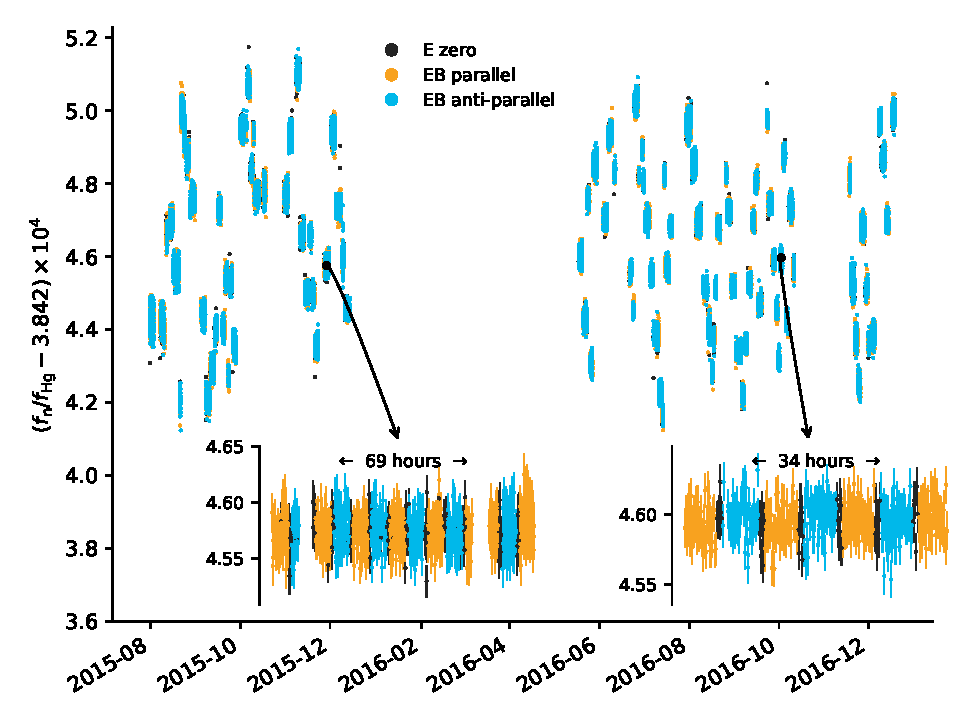
\includegraphics[width=0.9\linewidth]{gfx/axions/deltah4mm_time_domain_inset_no_yerr.pdf}
  \caption{The complete PSI data set used in the analysis. It spans from July 2015 to December 2016. Two sequences are enlarged. Due to high density of the measurements individual points cannot be resolved. The colours depict the relative orientation of the magnetic and electric fields: $E \uparrow \uparrow B$ (orange), $E \uparrow \downarrow B$ (blue) and $E=0$ (black). The $R$ time series has been corrected for gradient drifts. In the insets the points are draw.}\label{fig:PSI_dataset_time_domain}
\end{figure}

The data used in the analysis were collected at PSI between 2015--07--03, 14:21:30 and 2016--12--18, 19:51:23. The measurements were performed primarily to obtain the estimate of the constant nEDM\@. The time series of the ratio of the precession frequencies of the neutrons and mercury atoms $R = \nu_\text{n} / \nu_\text{Hg}$ is presented in Fig.\,\ref{fig:PSI_dataset_time_domain}.

\marginpar{A technical term for uninterupted operation was a run. Sometimes a run was stopped due to technical reasons a new started afterwards. A sequence combines those consecutive runs, that could be one run if not for the interruption.}
Take a look first at the inset in the lower-right corner. It zooms into data collected within one \emph{sequence}, typically 1--3 days long.
During a sequence the apparatus completed one cycle after another, one every \SI{300}{\second}, each yielding an estimate of $R$.
The electric field was automatically changed between three states: pointing upwards, being zero and pointing downwards. The different relative orientations of the electric and magnetic fields are depicted in colour in the figure. Sometimes there were technical breaks in the data taking during a sequence, as in the case of the one shown in the lower-left corner of Fig.\,\ref{fig:PSI_dataset_time_domain}.

% Here what it is and what's done Sometimes the automatic process was interrupted, but the sequence still continued, as seen in the other inset.

% REFER TO WHAT WAS IN HOW THE SIGNAL WOULD LOOK LIKE! But, repeating a bit will not hurt. The reader should already be prepared, now just reiterate.

% \mnote{Idea: present a scheme of the timing structure of the nEDM data taking, where a cycle, sequence are defined, and HV and B field reversals are shown.}
% The time structure ias follows: The atomic measurement is called a cycle, which gives an estimate of the average precession frequency of the neutrons $f_\mathrm{n}$ and mercury $f_\mathrm{Hg}$. Their ratio $R = f_\mathrm{n} / f_\mathrm{Hg}$ is show in Fig.\,\ref{fig:PSI_dataset_time_domain}. An automatic system executes one cycle after another (triggered on a signal from the UCN source). A series of automatically executed cycles is called a \emph{run}. The $R$ time series of a typical run, 1-3 days long, is shown in the lower-right corner. During a run the electric field automatically changes polarity every \ldots \mnote{Find out how many cycles for one HV cycle} cycles. In between \ldots cycles with no electric field are measured. These have no sensitivity to the electric dipole moment, but provide a control data set.

A sequence was taken always in one magnetic field configuration. The in-sequence variations of the vertical gradient of the magnetic field $\partial_z B_z$ were corrected for using the field model fits to the readings of the Caesium magnetometers. In between the sequences the vertical gradient was changed in \SI{10}{\pico\tesla} steps, up to \SI{60}{\pico\tesla}, so that those systematic effects, which scale linearly with the gradient, could be extrapolated to zero (see Sec.\,\ref{sec:measurement_procedure}). These large changes in the vertical gradient caused the large shifts in $R$ from sequence to sequence.

The $R$ time series was sliced into three separate based on the relative direction of the magnetic and electric fields: $E \uparrow \uparrow B$, $E \uparrow \downarrow B$ and $E=0$. In each a search for a harmonic oscillation was performed.

% During a single run the magnetic field is kept as stable as the team can manage. The drifts of the homogeneous part of the field are cancelled in $R$, but the gradients are not. So drifts of the gradient directly cause changes in $R$. These, however, can be corrected for using the Cs magnetometers. They are mounted on the top and bottom electrode and they can be used to correct for the in-run gradient drifts. They do not provide an accurate measure of the gradient. \mnote{Remember the reasoning why the cross-run gradient-drift correction can't be done: to large a change and the calibration issues}.

% Sometimes for technical reasons there is a pause in the measurements. Then the collected data may still belong to one run One such sequence is shown in the lower-right inset in Fig.\,\ref{fig:PSI_dataset_time_domain}.

% Typically... Sometimes stopped... Define a sequence



% Really, really first, show some example runs. 



\section{The analysis itself}
\begin{figure}
  \centering
  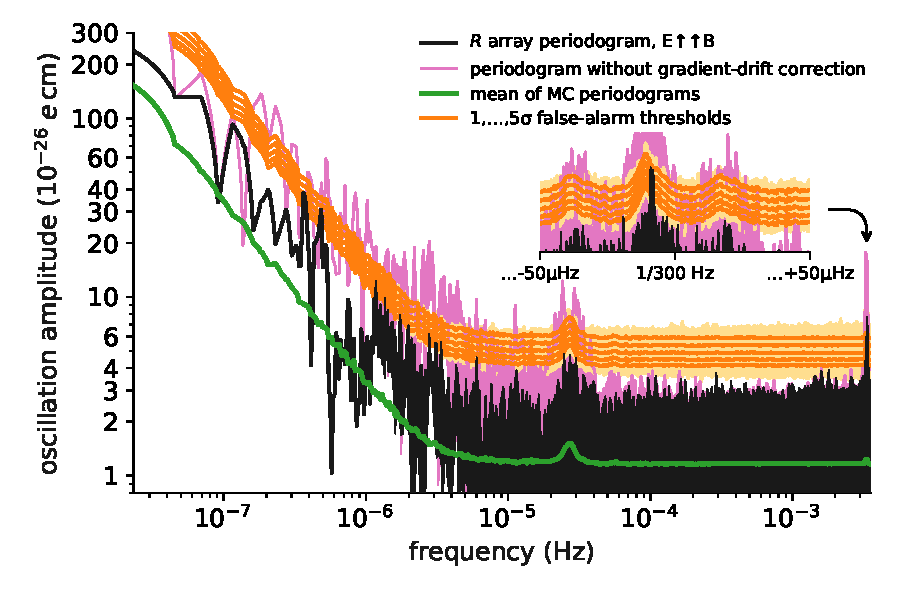
\includegraphics[width=0.9\linewidth]{gfx/axions/detection_psi_inset_gc.pdf}
  \caption{Periodogram of the $R$ time array of the PSI experiment data, sensitive to oscillations in the quantity $d_\mathrm{n} - \left( \mu_\mathrm{n} / \mu_\mathrm{Hg} \right) \, d_\mathrm{Hg}$, taken with the $\boldsymbol{E}$ and $\boldsymbol{B}$ fields parallel (black line).
  The mean of MC-generated periodograms, assuming no signal, is depicted in green. MC is used to calculate $1,2,…,5\,\sigma$ false-alarm thresholds, depicted in light orange.
  For clarity, we also plot the smoothed version in orange.
  There are two regions where a rise in the amplitude is expected, namely around \SI{28}{\micro\hertz} (inverse of 10 hours) and \SI{3.3}{\milli\hertz} (inverse of 300 seconds), due to the time structure of the data taking (see the main text for more details). The periodogram of non-gradient-drift-corrected data is shown in pink.}\label{fig:axions_PSI_detection}
\end{figure}

The periodogram of the subset of data with the electric and magnetic field parallel $E \uparrow \uparrow B$ is presented in Fig.\,\ref{fig:axions_PSI_detection} in black. The average null-hypothesis periodogram is depicted in green and the false-alarm thresholds in orange. An inset details the region around inverse \SI{300}{\second}, the cycle frequency.

There are two regions of expected rise in the oscillation amplitude due to the time structure of the data collection.
\marginpar{Recall the discussion in Sec.\,\ref{sec:a_null_hypothesis_test} about the peaks in the periodogram solely due to the time structure of the series.}
The one around \SI{28}{\micro\hertz} (the inverse of 10 hours) corresponds to the period of the reversal of the electric field.
The other, around \SI{3.3}{\milli\hertz}, the inverse of \SI{300}{\second}, corresponds to the cycle repetition rate.

The periodogram of the $R$ time array without the gradient-drift correction is shown in pink in Fig.\,\ref{fig:axions_PSI_detection}. The correction had an effect only for frequencies slower than the period of the reversal of the electric field (the region around inverse \SI{300}{\second}, the cycle frequency, is also sensitive to slow oscillations). The period of the electric field change had been deliberately chosen such, that was possibly infrequent (it took \note{how much} to ramp), but still occurring when the magnetic field had not drifted significantly away.

In the periodogram of the gradient-corrected time series here are five
%\note{NA does anybody know what style guide says about when numbers should be written in words i.e. seven vs 7? I personally think small numbers without units should be words but this comes down to preference} ***I THINK LESS THAN TEN IT IS IN WORDS - MALCOLM ***
trial frequencies for which the $3\upsigma$ false-alarm threshold is exceeded,
%\note{PMM: use words like 'surpassed', or 'exceeded' instead of penetrated}
two of which, including the largest excess with a $6\upsigma$ significance, occur in a \SI{100}{\micro\hertz} region around the inverse of \SI{300}{\second}, while the other three are in the low-frequency region, longer than an inverse length of a sequence.
% \note{FP: Can you maybe also explicitly state the positions of these three lines in Hz or inverse time?}
 The periodograms for the other two datasets, very similar to this one, can be found in App.\,\ref{ch:alp_appendix}.
In the other sensitive set, there are three excesses of the $3\upsigma$ threshold (the highest is $5\upsigma$), all constrained to the same two regions. In the control dataset, only the $1\upsigma$ threshold is exceeded. Among those, none fulfill the detection criteria, in particular the requirement to be present in both $E \uparrow \uparrow B$ and $E \uparrow \downarrow B$ periodograms, with opposite phases.
%\note{MR: We may consider not discussing the false--alarm threshold penetrations, and just state in the next paragraph that we do not find a signal which meets our criteria.}

% \mnote{Here a brief discussion about the Cs-gradient-drift correction.}
% It is interesting to observe, that the periodograms with and without the gradient drift correction diverge only for frequencies below \SI{6e-5}{\hertz}, the period of the high-voltage reversal (the disagreement around inverse \SI{300}{\second} is folded from the low frequencies). This is not a coincidence. The period of the high-voltage reversal has been deliberately chosen, so that\ldots\mnote{Was the period really chosen such?}

\begin{figure}
  \centering
  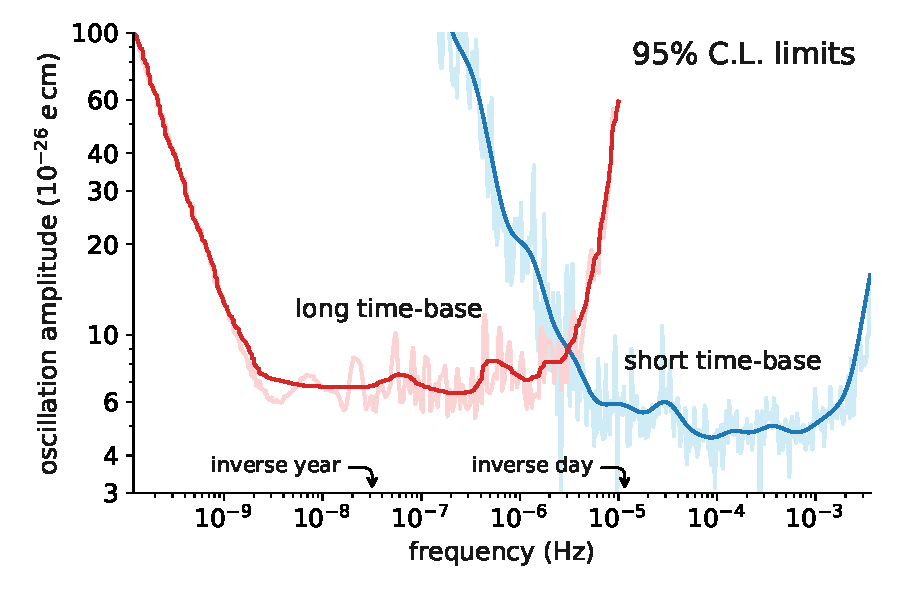
\includegraphics[width=0.8\linewidth]{gfx/axions/psi_ill_1e-26ecm.pdf}
  \caption{Limits on the amplitude of oscillation in the quantity $d_\text{n} - \frac{\mu_\text{n}}{\mu_\text{Hg}} \, d_\text{Hg}$, as a function of frequency thereof. The are above the curves is excluded on the 95\% C.L. The limit of this analysis (of the PSI data) are depicted in blue; the red curve depicts the limits of the complimentary analysis of the ILL-based experiment's data~\cite{AyresThesis,PhysRevX.7.041034}. The numerically obtained limits are depicted with faint lines; the bold lines are smoothed.}
\label{fig:axions_limits_nEDM}
\end{figure}

As no significant signals have been observed, limits could be placed to exclude the observations that would have been detected. The limits, obtained numerically in a way discussed in Sec.\,\ref{sec:signal_hypotheses_tests}, are depicted in Fig.\,\ref{fig:axions_limits_nEDM} in blue (labelled ``short time-base''). This analysis was most sensitive for periods between the duration of a sequence, around two days, and cycle repetition, \SI{300}{\second}. In that region amplitudes down to \SI{5e-26}{\elementarycharge\centi\meter} could be excluded on the 95\%~C.L. The limits of the long time-base analysis, the one of the ILL-based experiment's data~\cite{AyresThesis,PhysRevX.7.041034}, are depicted in red. Complimentarily, they are sensitive to periods just below the duration of a sequence and go down to about a decade.

\begin{figure}
  \centering
  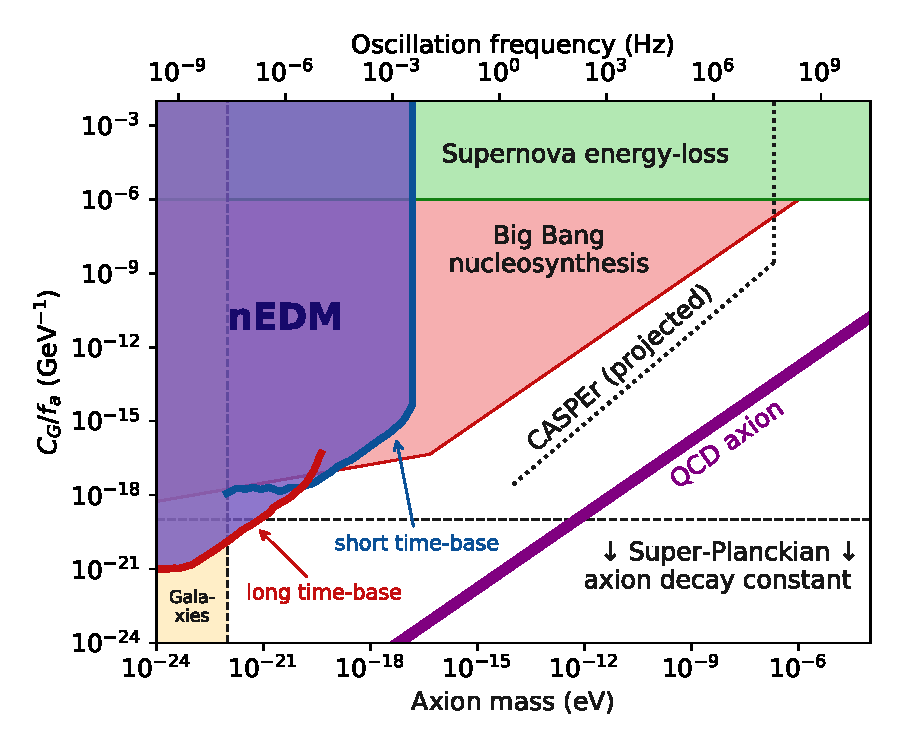
\includegraphics[width=0.8\linewidth]{gfx/axions/psi_ill_axion_limits_v7.pdf}
  \caption{Limits on the interaction of an axion with the gluons (95\% C.L.). Tha parameter space is spanned by the axion's mass (horizontal) and the strength of the coupling (vertical). It has been assumed, that axions saturate the local cold dark matter density. Other depicted constraints are: Big Bang nucleosynthesis (red, 95\% C.L.)~\cite{Blum2014,StadnikThesis,Stadnik2015D}, supernova energy-loss bounds (green, order of magnitude)~\cite{Graham2013,Raffelt1990Review,Raffelt2008LNP}, consistency with observations of galaxies (orange)~\cite{Marsh2015Review,Marsh2015B,Schive2015,Marsh2017}. The projected reach of the proposed CASPEr experiment is depicted with a dotted black line~\cite{CASPEr2014}, and the parameter space for the canonical QCD axion with a purple band.}
\label{fig:axions_limits_coupling}
\end{figure}

Following the Eq.\,(\ref{eq:nEDM_axion}), the oscillating-nEDM limits were interpreted as ones on the axion-gluon coupling. The results are presented in the axion space, spanned by their mass and the strength of the coupling, in Fig.\,\ref{fig:axions_limits_coupling}. These first laboratory constraints are presented in the landscape of already existing cosmological limits: axions with a mass below \SI{1e-22}{\electronvolt} have their Compton wavelength larger than the size of the smallest dwarf galaxies and, therefore, could not be the sole constituent of dark matter~\cite{Marsh2015Review}; the influence of axions in the red-shaded area on the Big Bang nucleosynthesis would result in an underproduction of ${}^4$He~\cite{Blum2014}; the green area was excluded based on the observations of the supernova SN1987A, where excess cooling by axion emission would have been observed~\cite{Graham2013}.


% The Fig.\,\ref{fig:axions_limits_coupling} features the \emph{short time-base} limits, the ones described in this work, as well as \emph{long time-base} ones.
% This work was performed with close collaboration with Nicholas Ayres of the University of Sussex. The Sussex group was part of the collaboration running the predecessor of the nEDM experiment at PSI --- the measurement performed in the Institute Laue-Langevin in Grenoble, France, in the years 1998--2002~\cite{Pendlebury2015}.
% An analysis analogous to this work was performed on those data, with an important difference, which made it sensitive to lower frequencies (or lighter axions)~\cite{AyresThesis}.
% Namely, the time series consisted of one point per run, in contrast to one per cycle in the short time-base analysis.
% On one hand it limits the sensitivity to oscillation periods corresponding to one run (1--2 days).
% On the other, the sensitivity to low frequencies is not deteriorated, as there is no need to use multiple free offsets in the LSSA fit (Eq.\,(\ref{eq:axions_LSSA})). In fact the free offset is assumed to be zero on the ground that the experiment delivered a zero-compatible result.
% % in the process of calculating the per-run nEDM estimate the gradient fluctuations are averaged out, so there is 
% \mnote{What about the gradient-related systematics (nEDM vs R' curve)? Was it corrected for? Wrote an email to Nick.}

% Despite close collaboration the two analyses shared no common code. As a mean of cross-check, the two codes were compared on artificial datasets, more on that in the appendix.




\section{Axion-Wind analysis}
The analysis described so far was concerned with the scalar coupling of the axions to gluons, which looks like an oscillation in the electric dipole moment of the neutron.
The same data set, and the same analysis techniques, were also used for a different coupling---a vector one of axions to nucleons. This coupling acts like an additional dynamic magnetic field, so the data were split based on the direction of the holding magnetic field $B_0$, as indicated in Fig.\,\ref{fig:axions_wind_time_domain}. The axion-wind coupling is insensitive to the electric field in the experiment.

\begin{figure}
  \centering
  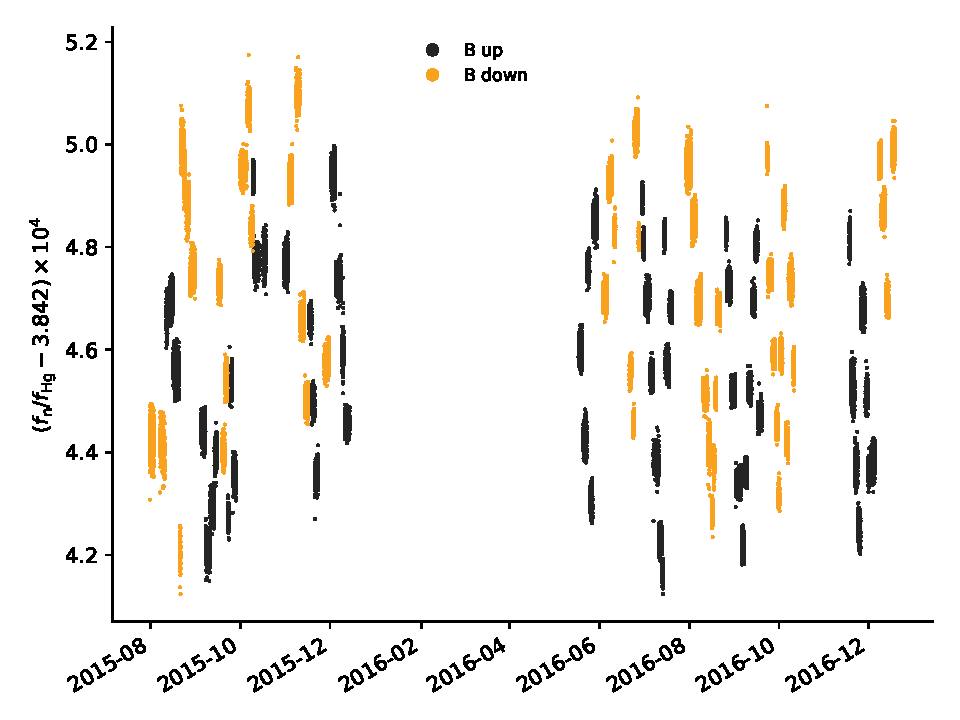
\includegraphics[width=0.9\linewidth]{gfx/axions/wind_winddeltah4mm_time_domain_inset_no_yerr.pdf}
  \caption{The $R$ time series measured at PSI measured between July 2015 and December 2016 with the orientation of the magnetic field marked. The two orientations form the two datasets for the axion-wind analysis.}\label{fig:axions_wind_time_domain}
\end{figure}

The coupling, Eq.\,\ref{potential_axion-wind}, is proportional to the projection of experiment's quantisation axis on the momentum of the axions.
Because the latter arises due to the Earth's traversing the galactic axion field in the Solar System's movement around the Milky Way's centre, the effect is called the axion-wind~\cite{Stadnik2014A}.
The Earth additionally spins, causing the effect to be modulated with the sidereal frequency $\Omega_\text{sid}$, equal to \num[detect-all=true]{23.9344699} hours. \note{ref needed}
\marginpar{Sidereal frequency is the one of the Earth's spinning as seen in the reference of distant stars.}
The modulation would have made a signal in periodogram a triplet, with the central, highest, peak at the frequency of the oscillation of the axion field, and two additional ones on either side, $\Omega_\text{sid}$ away from the main peak.

There were two datasets, with the magnetic field pointing in either way along gravity, both sensitive to the effect. The periodograms are presented in Fig.\,\ref{fig:axions_wind_detection}. There are 44 frequencies with power above the 3$\upsigma$ threshold in $B\uparrow$ and 36 in $B\downarrow$, but there are only two frequencies where the threshold is exceeded in both data sets simultaneously: \SI{3.42969}{\micro\hertz} and \SI{3.32568}{\milli\hertz}. Neither of the signal fulfilled the requirement of the phase being opposite in the two data sets.

\begin{figure}
  \centering
  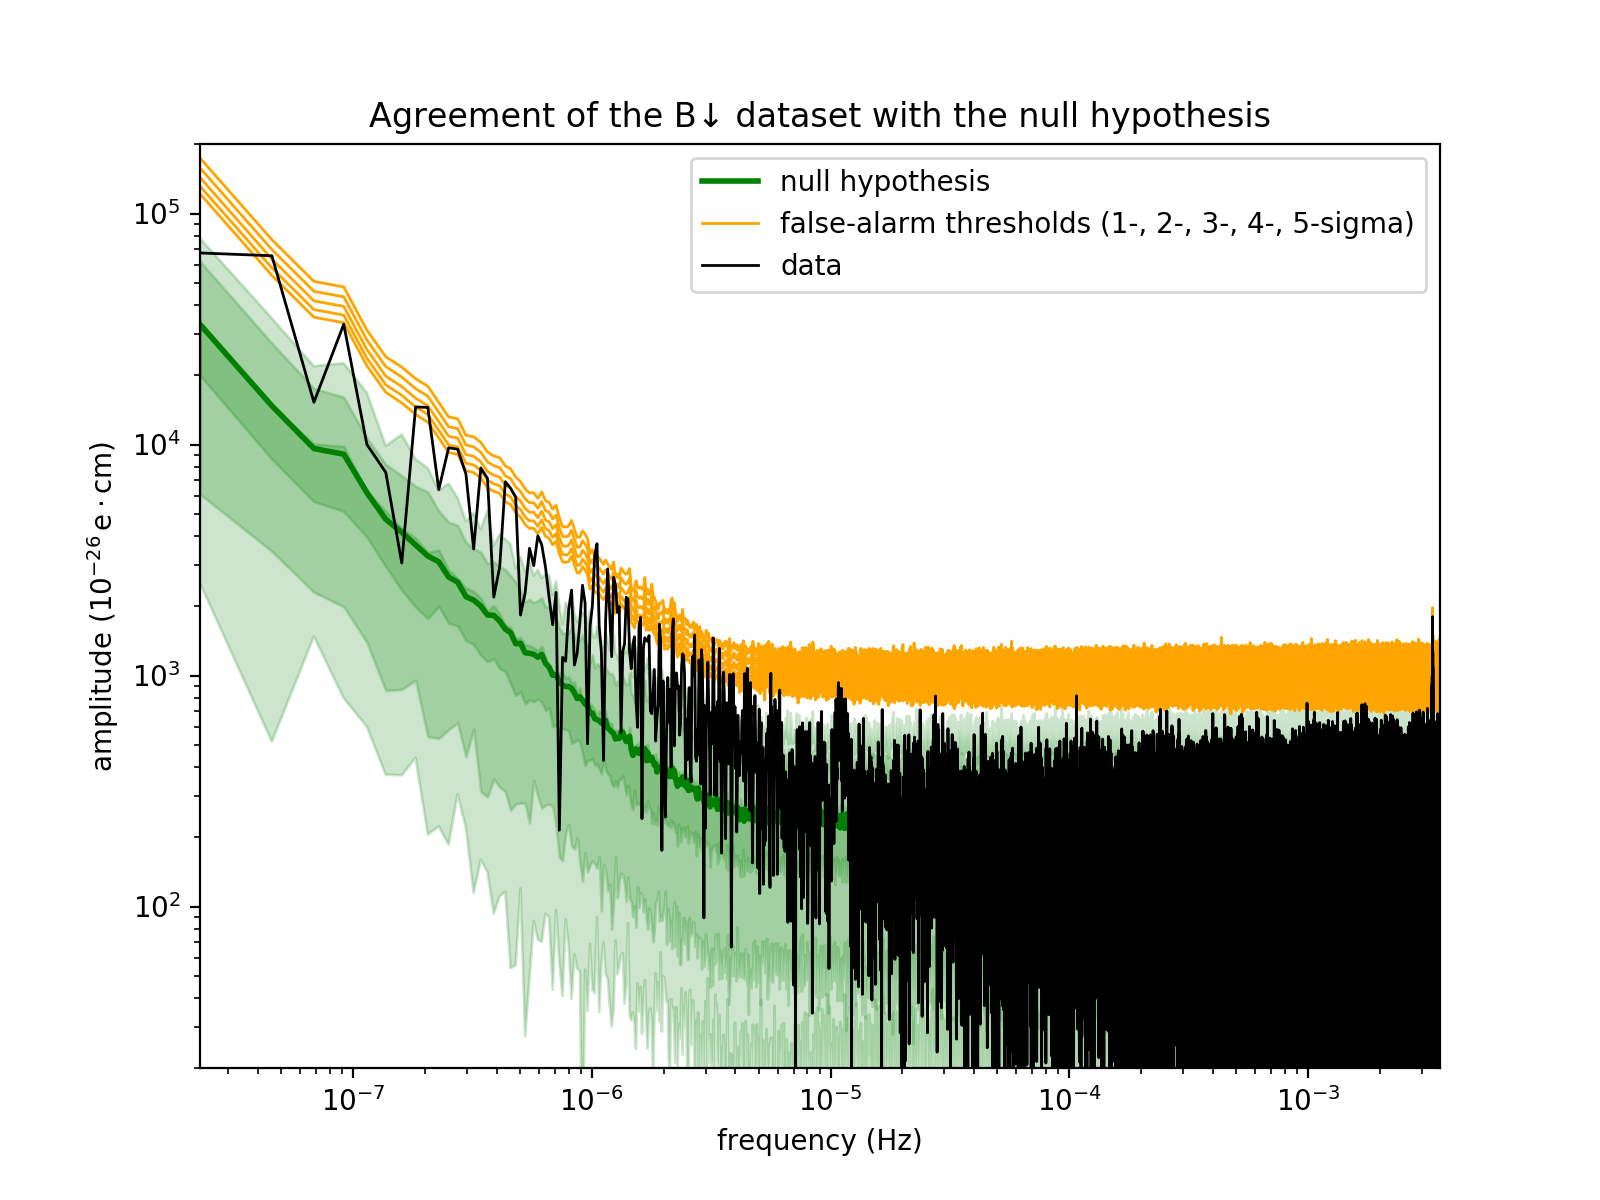
\includegraphics[width=0.9\linewidth]{gfx/axions/winddeltah4mm_Bdown_detection.png}
  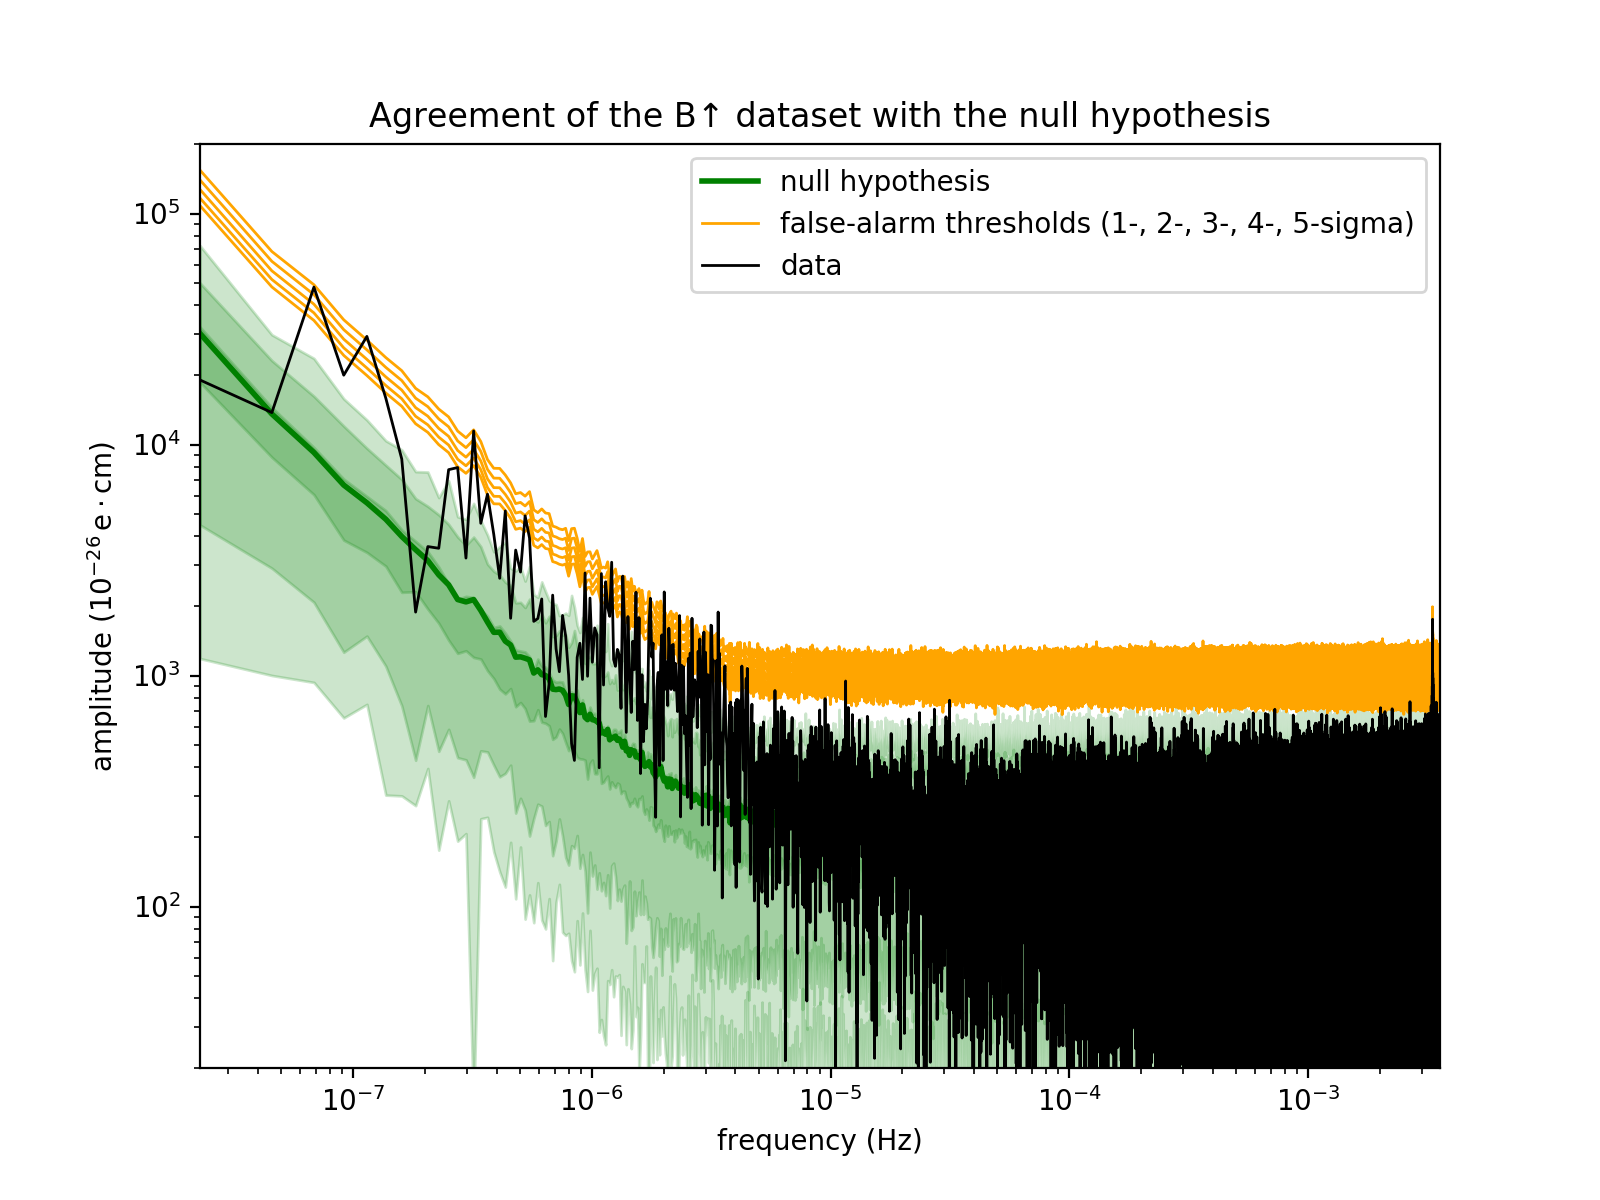
\includegraphics[width=0.9\linewidth]{gfx/axions/winddeltah4mm_Bup_detection.png}
  \caption{The periodogram of the $R$ time series measured with the main magnetic field pointing upwards. The distribution of MC-generated periodograms, assuming no signal, is depicted in green (the 1, 2 and 3$\upsigma$ bands and the mean with a line). The 1,2,…,5$\upsigma$ false-alarm thresholds are depicted in orange.}\label{fig:axions_wind_detection}
  % For clarity, we also plot the smoothed version in orange.}
\end{figure}

% \begin{figure}
%   \centering
%   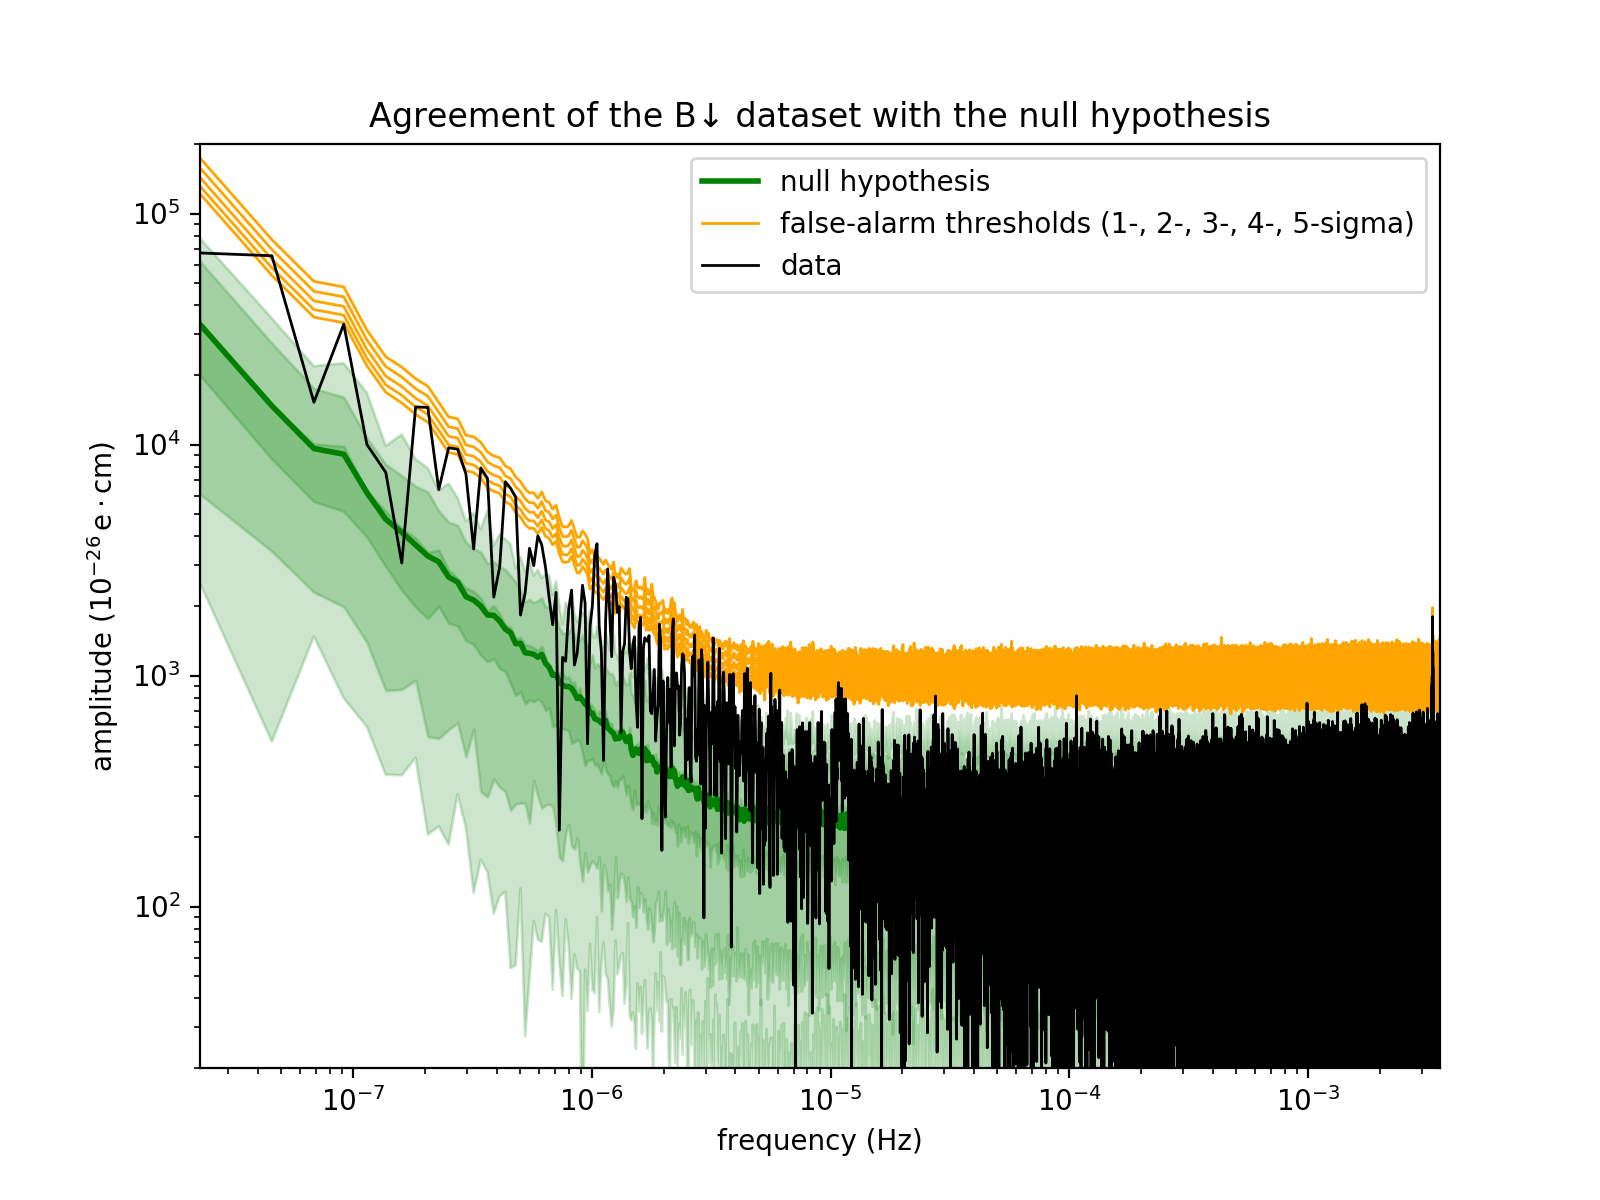
\includegraphics[width=0.9\linewidth]{gfx/axions/winddeltah4mm_Bdown_detection.png}
%   \caption{\ldots}\label{fig:axions_wind_detection}
% \end{figure}

The lack of statistically significant signal compatible with the axion model allowed us to put limits on the axion-nucleon coupling, depicted in Fig.\,\ref{fig:axions_wind_limits}. \note{comment a bit on the other limits in the plot}

\begin{figure}
  \centering
  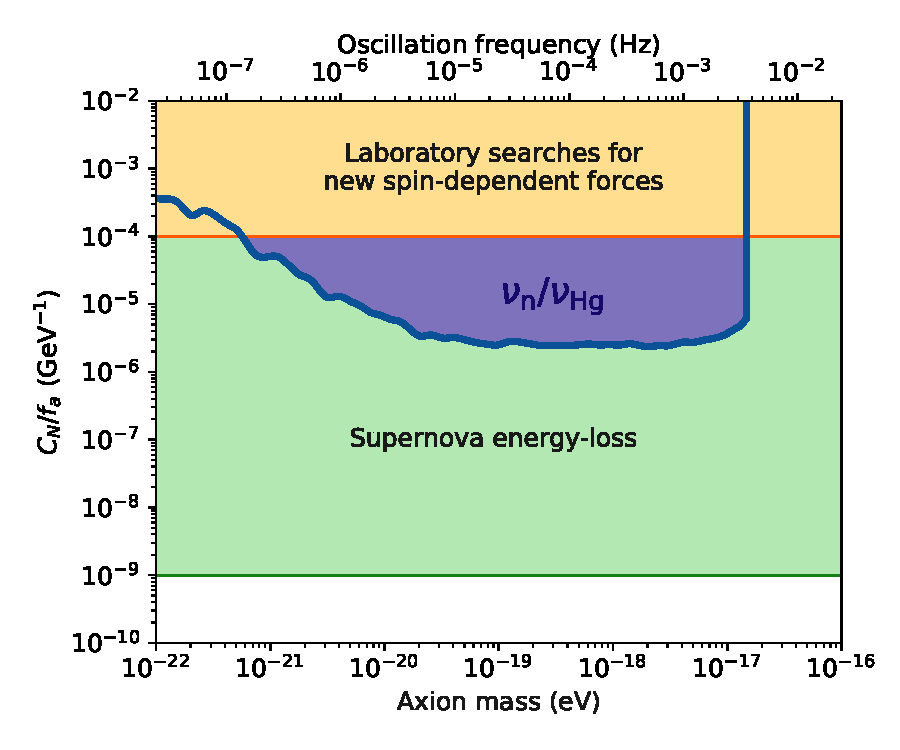
\includegraphics[width=0.8\linewidth]{gfx/axions/psi_ill_axion_wind_limits_v1.pdf}
  \caption{Excluded regions of the space of the coupling of axions to nucleons (Eq.\,\ref{potential_axion-wind}). The green region is excluded from observations of the SN1987A supernova~\cite{PhysRevX.7.041034}, and the yellow one from K--${}^3$He magnetometry~\cite{Romalis2009_NF}. The blue region, is the exclusion arising from this analysis.}\label{fig:axions_wind_limits}
\end{figure}




\section{Sidereal frequency}
\begin{figure}
  \centering
  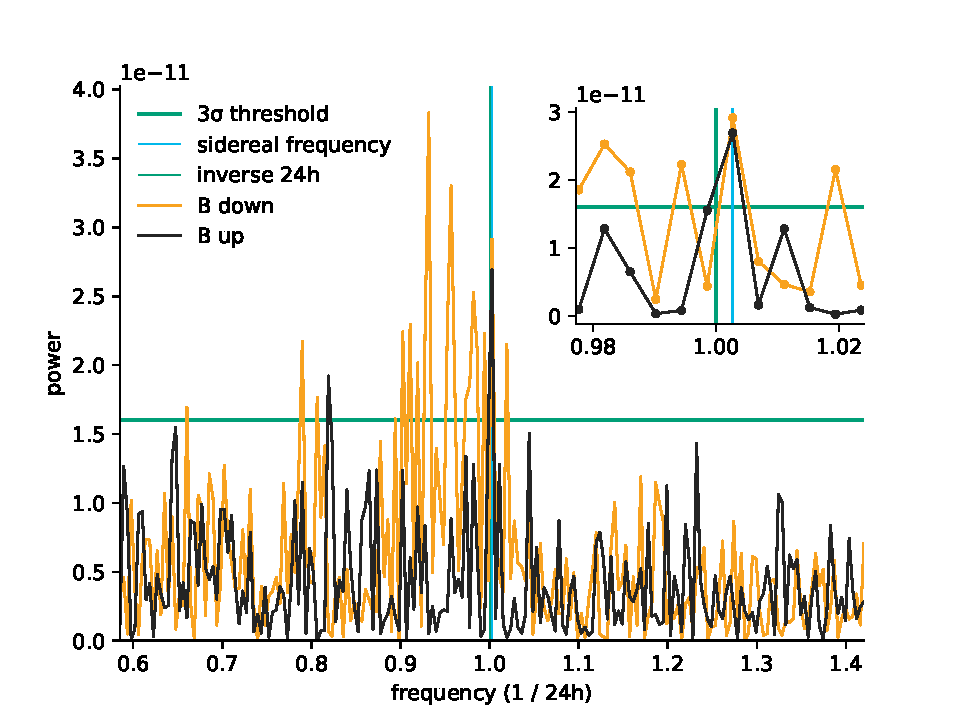
\includegraphics[width=0.8\linewidth]{gfx/axions/winddeltah4mm_sidereal.pdf}
  \caption{\cite{Romalis2009_NF}}\label{fig:axions_sidereal_detection}
\end{figure}

\begin{figure}
  \centering
  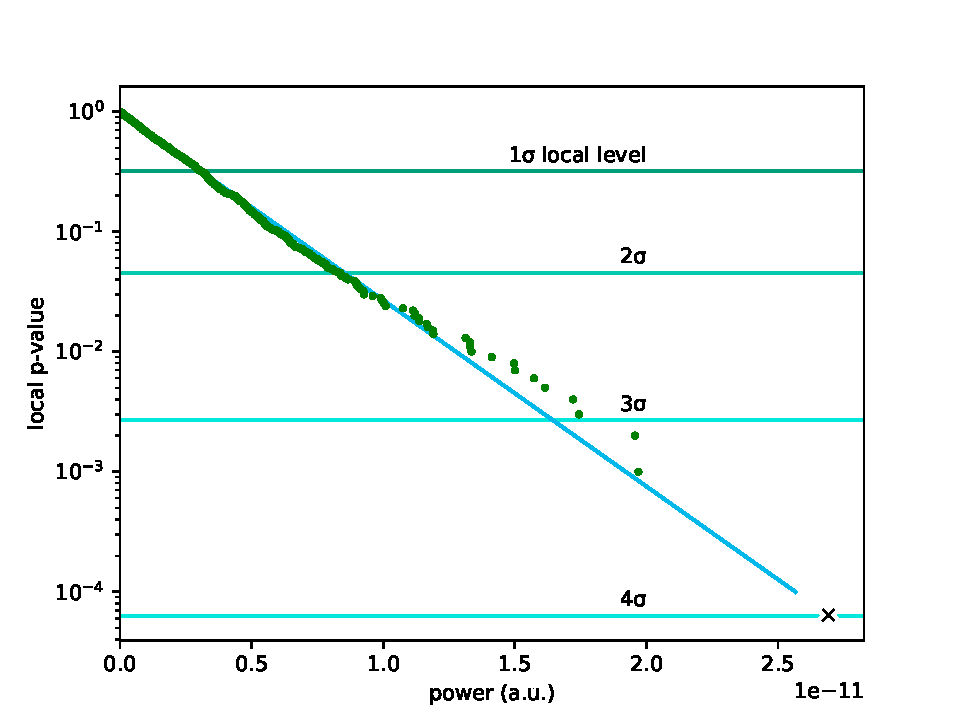
\includegraphics[width=0.8\linewidth]{gfx/axions/winddeltah4mm_sidereal_detection.pdf}
  \caption{\cite{Romalis2009_NF}}\label{fig:axions_sidereal_cdf}
\end{figure}

A note about the signals seen at this particular frequency. Refer to the Lorentz-invariance paper, improve the limit directly?~\cite{ALTAREV20112365}

Another magnetic-field-like effect\ldots

At the moment (21 Feb 2018) it seems, that there is a signal exactly at the sidereal frequency. The periodograms are in Fig.\,\ref{fig:axions_sidereal_detection}. It is around 4$\upsigma$ in both datasets, the CDF of the B up dataset is in Fig.\,\ref{fig:axions_sidereal_cdf}. The phase relation is correct (around \ang{160}, but I don't know the uncertainty on that number). In the B up dataset it sticks prominently out exactly there. In the B down dataset it is a bit problematic, as this happens to be right at the edge of some wider excess in power, so this peak is surrounded by a couple more, some even more significant. I could cut the data to get this peak out. 



\section{Outlook}
There are three direction in which the nEDM-based axion dark matter search could continue.
To improve sensitivity vertically (be sensitive to more weekly coupled or less abundant axions) the overall sensitivity of the nEDM measurement would need to be improved.
Following the Eq\,\ref{eq:nEDM_sensitivity}: more neutrons, higher electric field or longer precession time.
% \marginpar{In Eq\,\ref{eq:nEDM_sensitivity} $\alpha$ is already \ldots, precession time $T$ can only be improved so long---it is fundamentally limited by the neutron life-time (give the number.)}
The global community already spares no effort in this respect.

The second way is to improve sensitivity for slower oscillations, or lighter axions, limited by the span of the data set---four years in the case of the ILL nEDM data set. Combining the ILL and PSI data into one time series would improve it to 19 years. It was not done at the time, because the PSI data were still blinded and analysis to obtain the nEDM time series, one like in the ILL dataset, was still ongoing. In any case, axions oscillating this slow would be so light, that their Compton wavelength would not fit in small dwarf galaxies~\cite{Marsh2015Review}, which rules them out as a single dark matter constituent.

The third direction is the high-frequency, heavy-axions one. It is limited by the sampling frequency fo the system, the cycle repetition rate. The measurements could be conducted with a shorter cycle time (worsening the sensitivity, as the loss in Eq.\,\ref{eq:nEDM_sensitivity} is linear, and the gain from the improved statistics scales with the square root).
\marginpar{At PSI the cycles were synchronised to the pulses of a kicker magnet, which redirected a proton beam onto the target of the UCN source.}
However, it is hard to imagine going beyond ten-second range. A real improvement in this direction would require changing the principle of the measurement.




\section{Resonant oscillating nEDM search}
Both searches that have been discussed, were what is called broad-band. The measurement are sensitive to a wide range of frequencies. In contrast to that, resonant searches, like ADMX~\cite{PhysRevLett.104.041301} or proposed CASPEr~\cite{CASPEr2014}, are sensitive at a any given time only to a relatively narrow band of frequencies. Covering a wide range requires scanning. In this section a resonant search of an oscillating nEDM is proposed.

% Many of the axion searches are resonant based.~\cite{PhysRevLett.104.041301,CASPEr2014} \note{some references}.
% The standard instrument to look for an axion-photon coupling, called a haloscope \note{verity}, consists of ultra-low-noise resonant cavity, where axions can produce photons, detected with an antenna \note{is it an antenna?}.
% At any given time the measurement is sensitive only to a narrow band of photon energies (or frequencies), the width given by the finesse \note{verity} of the cavity. To cover a wide range the tuning of the cavity is scanned. In this section an idea of a resonant oscillating nEDM search is pursued.

For polarised neutrons in a magnetic field, a transverse oscillating coupling induces a coherent Rabi oscillation between the spin-up and spin-down states.
For example, a Ramsey cycle begins with a $\uppi/2$ flip induced by an oscillating transverse magnetic field, its frequency tuned to the Larmor one and its length tuned such, that the Rabi oscillation stops when the polarisation is in the transverse plane. Should the nEDM oscillate, an oscillating transverse coupling can be realised with a static magnetic field \emph{perpendicular} to the holding magnetic field $B_0$. Then, if the frequency of the nEDM oscillation is tuned to the Larmor one, the neutrons would undergo a Rabi nutation, which could be detected.

\begin{figure}
  \centering
  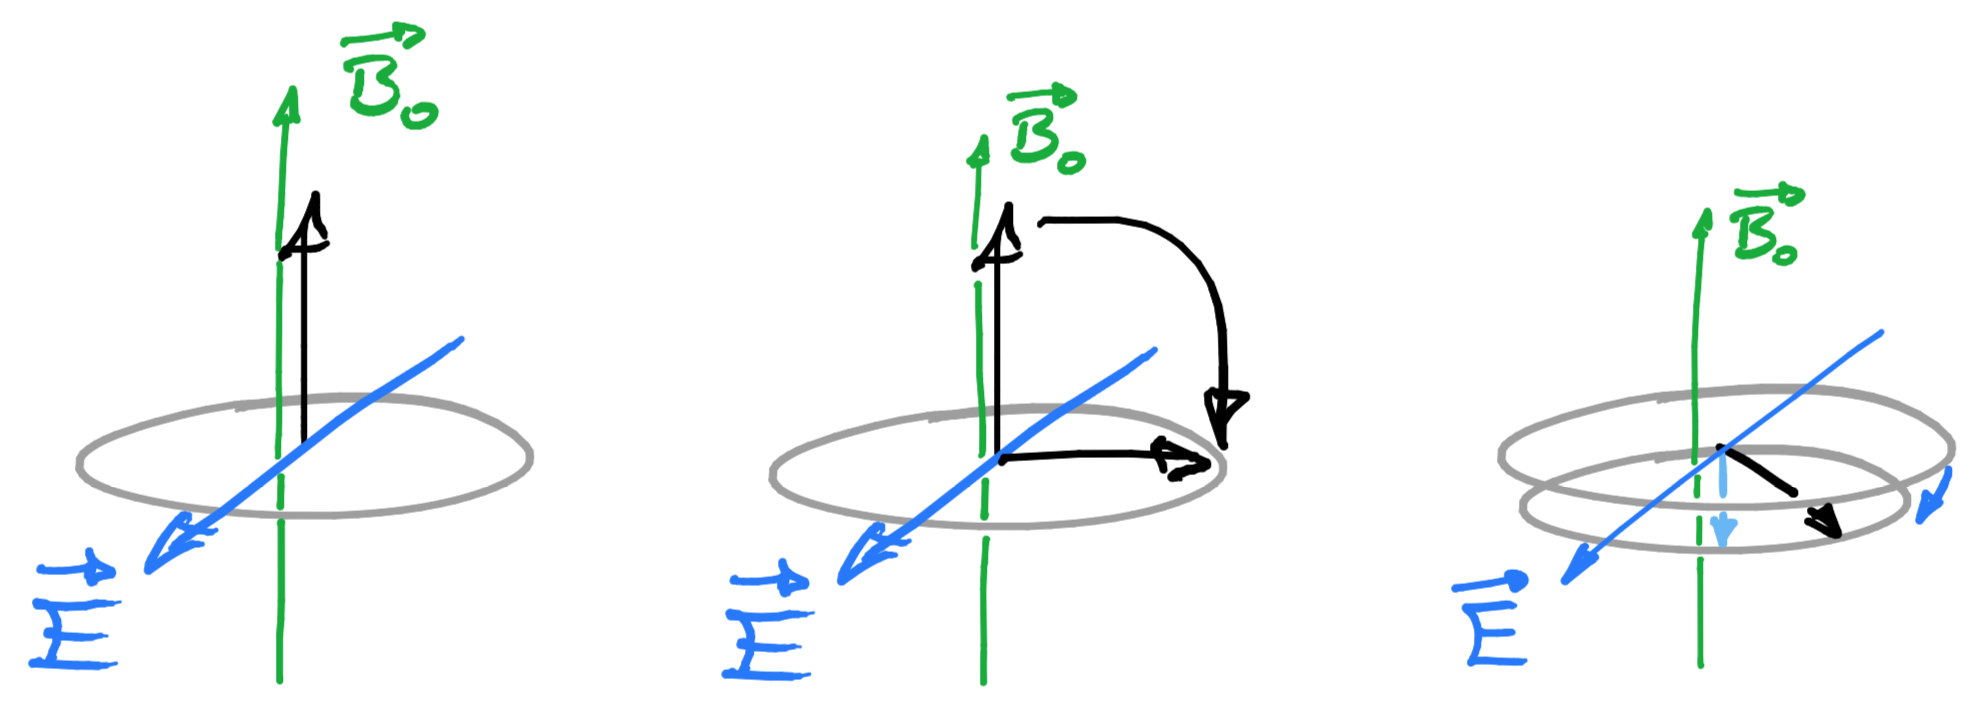
\includegraphics[width=0.8\linewidth]{gfx/axions/resonant_effect.png}
  \caption{The behaviour of the spin population in a resonant oscillating EDM search. One starts with an ensemble polarised along the holding magnetic field $B_0$. The electric field is perpendicular. Then, the polarisation is flipped by $\pi$/2 and starts the Larmor precession. The combination of the electric field and an oscillating EDM would induce a Rabi nutation. The direction of the nutation is determined by the relative phase of the Larmor precession and the EDM oscillation.}\label{fig:axions_resonant_effect}
\end{figure}

In the proposed scheme, sketched in Fig.\,\ref{fig:axions_resonant_effect}, the neutrons start polarised along the holding field and are put into the Larmor precession with a $\uppi/2$ flip. The oscillating nEDM would then induce a Rabi nutation and a net polarisation along the $B_0$ direction would build up, which could be measured. The direction of the nutation depends on the phase difference between the Larmor precession (defined by the phase of the $\uppi/2 pulse$) and the oscillating nEDM\@.

Sensitivity. \note{This I still need to calculate in detail.}
\begin{equation}
  H(t) = \bm{\mu} \cdot \bm - \bm{d}_\text{n}(t) \cdot \bm{E}
\end{equation}
In the Rabi precession we have an effective precession:
\begin{equation}
  H = - \bm{d}_\text{n}(t) \cdot \bm{E}
\end{equation}
field. The Rabi frequency is then:
\begin{equation}
  \chi = \frac{ \bm{d}_\text{n}(t) \cdot \bm{E} }{ \hbar }
\end{equation}
The rotation for a small angle is:
\begin{equation}
  \theta = \frac{ \bm{d}_\text{n}(t) \cdot \bm{E} }{ \hbar } \cdot T
\end{equation}
\note{Now somehow relate it to the nEDM sensitivity. What is the nEDM sensitivity to detect a polarisation in the UCN\@? Where do I get the additional factor of 2 from?}
\begin{equation}
  \sigma(d_\text{n}) = \frac{ \hbar }{ 2 \alpha E T \sqrt{N} }
\end{equation}

Additional factor $\sqrt{2}$ is lost due to the non-matching phases (on average). Two measurements done, with the Larmor precession (through the spin-flip pulses) shifted by \ang{90}, recover the full sensitivity.


Systematic effects: quality of the pi/2 pulse (all correlated with the electric field).

First---just scanning.

Broad band possibility? It is like an adiabatic spin-flip, but without the oscillating field. The fact that the spin flip occurs, would indicate a presence of the field.

\begin{figure}
  \centering
  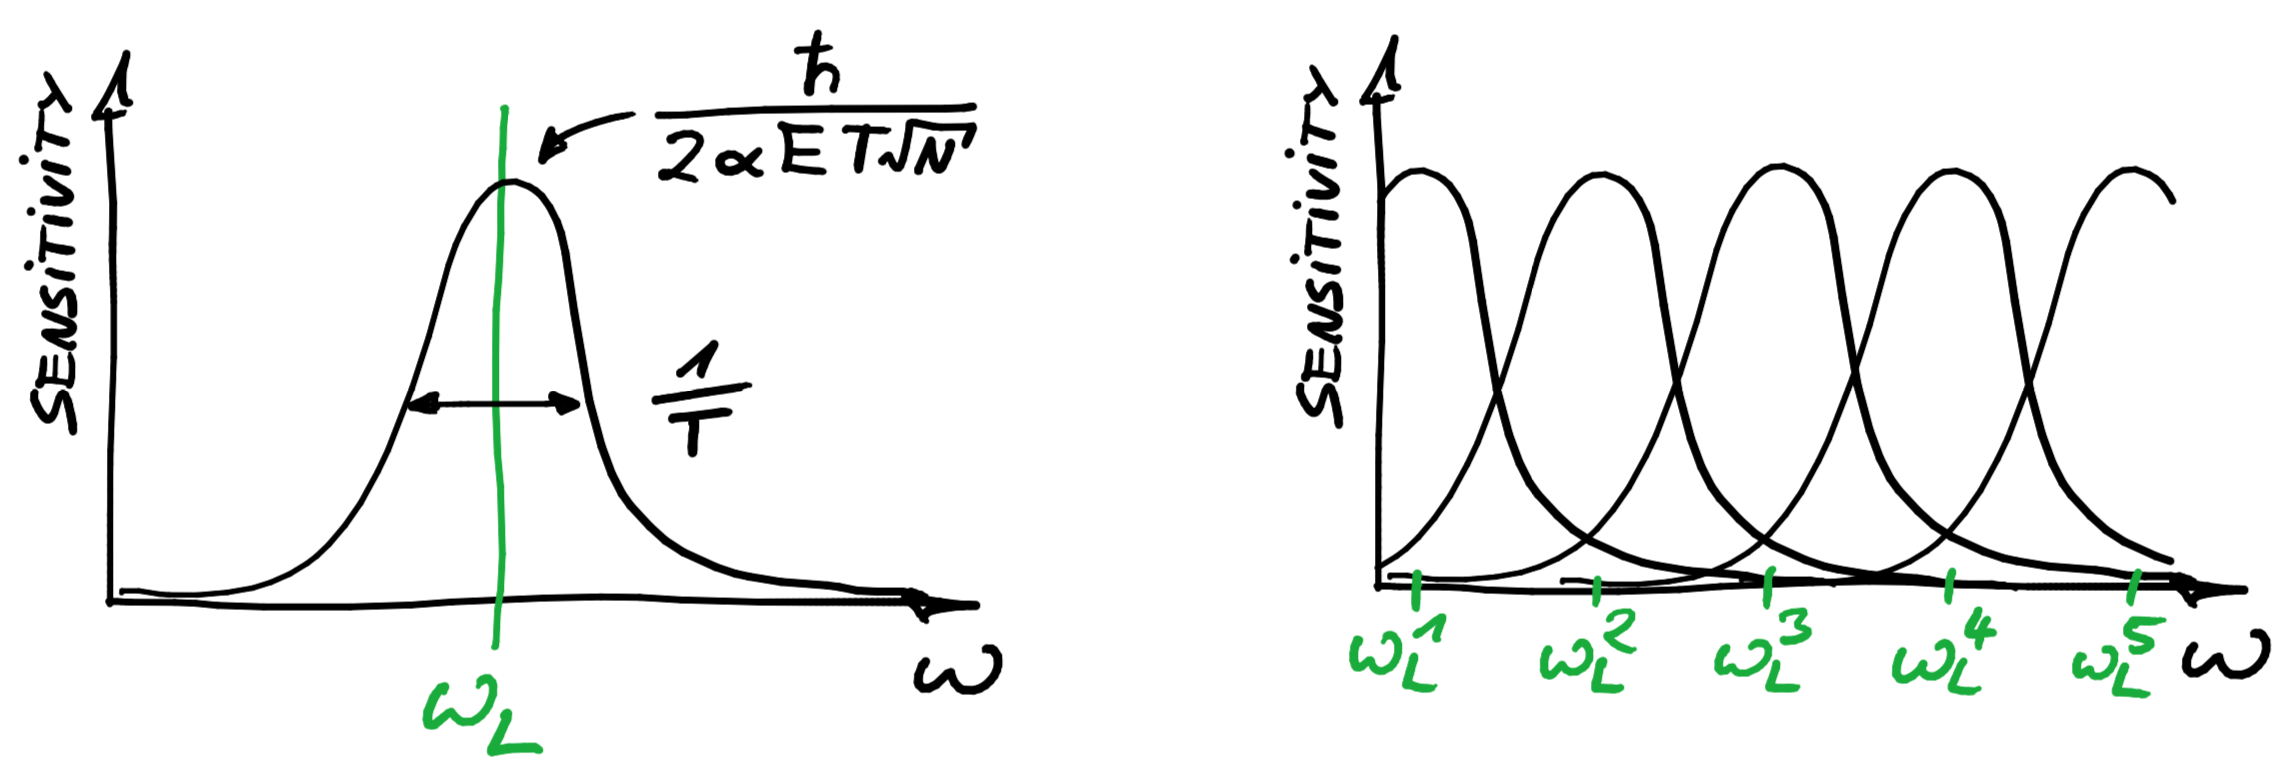
\includegraphics[width=0.8\linewidth]{gfx/axions/resonant_sensitivity.png}
  \caption{Left: the sensitivity of the resonant search has the width equal to the inverse interaction time. Right: a broad-band sensitivity needs to be built up with multiple measurements.}\label{fig:axions_resonant_sensitivity}
\end{figure}


\note{Some kind of summary here?}